% ---------------------------------------------------------------------
% -------------- PREAMBLE ---------------------------------------------
% ---------------------------------------------------------------------
\documentclass[12pt,a4paper,finnish,oneside]{article}
%\documentclass[12pt,a4paper,finnish,twoside]{article}
%\documentclass[12pt,a4paper,finnish,oneside,draft]{article}

\usepackage[utf8]{inputenc}

% Valitse 'output/font encoding':
%\usepackage[T1]{fontenc}      % korjaa ääkkösten tavutusta, bittikarttana
\usepackage{ae,aecompl}       % ed. lis. vektorigrafiikkana bittikartan sijasta

% Kieli- ja tavutuspaketit:
\usepackage[english,swedish,finnish]{babel}

% Kurssin omat asetukset aaltosci_t.sty:
\usepackage{aaltosci_t}

% Muita paketteja:
%\usepackage{alltt}
%\usepackage{amsmath}
\usepackage{calc}      % käytetään laskurien (counter) yhteydessä (tiedot.tex)
%\usepackage{eurosym}   % eurosymboli: \euro{}
\usepackage{url}       % \url{...}
\usepackage{listings}  % koodilistausten lisääminen
%\usepackage{algorithm} % algoritmien lisääminen kelluvina
%\usepackage{algorithmic} % algoritmilistaus
\usepackage{hyphenat}
\usepackage{supertabular,array}  % useampisivuinen taulukko

% Strikethrough
\usepackage[normalem]{ulem}


% Monta lähdeluoetteloa
\usepackage{multibib}
\newcites{pri}{Lähteet}

% Lähteiden listaus ilman lähdeluoetteloa
\usepackage{bibentry}


% Tavutus.
%\hyphenation{vää-rin me-ne-vi-en sa-no-jen tavu-raja-ehdo-tuk-set}
\hyphenation{me-ne-tel-män me-ne-tel-mis-tä tar-kas-te-luun}
\hyphenpenalty=10000   % rangaistaan tavutuksesta, 10000=ääretön
\tolerance=1000        % siedetään välejä riveillä
% titlesec-paketti auttaa, jos tämän mukana menee sekaisin

% Tekstiviitteiden ulkoasu.
% Pakettiin natbib.sty/aaltosci.bst liittyen katso esim. 
% http://merkel.zoneo.net/Latex/natbib.php
% jossa selitykset citep, citet, bibpunct, jne.
\bibpunct{(}{)}{;}{a}{,}{,}    % a = tekijä-vuosi (author-year)
%\bibpunct{[}{]}{;}{n}{,}{,}    % n = numero [1],[2] (numerical style)

% Rivivälin muuttaminen:
\linespread{1.24}\selectfont               % riviväli 1.5
%\linespread{1.24}\selectfont               % riviväli 1, kun kommentoit pois

% ---------------------------------------------------------------------
% -------------- DOCUMENT ---------------------------------------------
% ---------------------------------------------------------------------

\begin{document}

\selectlanguage{finnish}
\pagestyle{plain}
\pagenumbering{arabic}

\author{Kim Dikert}

\title{Ketterien kehitysmenetelmien käyttöönotto suurissa organisaatioissa: Kirjallisuustutkimus}


% Otsikko tiivistelmään. Jos lisäksi engl. tiivistelmä, niin viimeisin:
\TITLE{Ketterien kehitysmenetelmien käyttöönotto suurissa organisaatioissa: Kirjallisuustutkimus}
\ENTITLE{\LaTeX{} template for Bachelor thesis with a pretty long title %
line which continues ynd continues}

% Jos tarvetta 2-osaiselle otsikolle:
%\title{\LaTeX{}-pohja kandidaatintyölle \\[5mm] Pitkiä rivejä kokeilun vuoksi.}
%\TITLE{\LaTeX{}-pohja kandidaatintyölle. Pitkiä rivejä kokeilun vuoksi.}

% Ohjaajan laitos suomi/ruotsi ja tarvittaessa eng (tiivistelmän kieli/kielet)
\DEPT{Tietotekniikan laitos}
%\DEPT{Tietotekniikan laitos}
%\DEPT{Institutionen för datateknik}
%\ENDEPT{Department of Computer Science Engineering}

% Vuosi ja päivämäärä, jolloin työ on jätetty tarkistettavaksi.
\YEAR{2012}
\DATE{XX. marraskuuta 2012}
%\DATE{31. helmikuuta 2012}
%\DATE{Den 31 februari 2012}
\ENDATE{November XX, 2012}

% Kurssin vastuuopettaja ja työsi ohjaaja(t)
\SUPERVISOR{Ma professori Tomi Janhunen}
\INSTRUCTOR{TkT Maria Paasivaara}
%\INSTRUCTOR{Ohjaajantitteli Sinun Ohjaajasi, ToinenTitt Matti Meikäläinen}
% DI       // på svenska DI diplomingenjör
% TkL      // TkL teknologie licentiat
% TkT      // TkD teknologie doctor
% Dosentti Dos. // Doc. Docent
% Professori Prof. // Prof. Professor
% 
% Jos tiivistelmä englanniksi, niin:
\ENSUPERVISOR{Professor (pro tem) Tomi Janhunen}
\ENINSTRUCTOR{Maria Paasivaara, D.Sc.}
% M.Sc. (Tech)  // M.Sc. (Eng)
% Lic.Sc. (Tech)
% D.Sc. (Tech)   // FT filosofian tohtori, PhD Doctor of Philosophy
% Docent
% Professor

\PAAAINE{Ohjelmistotuotanto ja -liiketoiminta}
\CODE{T3003}

\KEYWORDS{agile, ketterä, ohjelmistokehitys, organisaatiomuutos}

\ENKEYWORDS{agile, software development, large scale, transformation}

% Kaikki sivut laskettuna nimiölehdestä lähdeluettelon tai 
% mahdollisten liitteiden loppuun. --> Miten liitteet (esim. "20 + 5")?
\PAGES{XX}

% ------------------------ Nimiölehti ---------------------------------

%\thispagestyle{empty}
\maketitle

% -------------- Tiivistelmä / abstract -------------------------------

\setcounter{page}{2}
% Tiivistelmät tehdään viimeiseksi. 
%
% Tiivistelmä kirjoitetaan käytetyllä kielellä (JOKO suomi TAI ruotsi)
% ja HALUTESSASI myös samansisältöisenä englanniksi.
%
% Avainsanojen lista pitää merkitä main.tex-tiedoston kohtaan \KEYWORDS.

\begin{fiabstract}
  Tiivistelmä on muusta työstä täysin irrallinen teksti, joka
  kirjoitetaan tiivistelmälomakkeelle vasta, kun koko työ on
  valmis. Se on suppea ja itsenäinen teksti, joka kuvaa olennaisen
  opinnäytteen sisällöstä. Tavoitteena selvittää työn merkitys
  lukijalle ja antaa yleiskuva työstä. Tiivistelmä markkinoi työtäsi
  potentiaalisille lukijoille, siksi tutkimusongelman ja tärkeimmät
  tulokset kannattaa kertoa selkeästi ja napakasti. Tiivistelmä
  kirjoitetaan hieman yleistajuisemmin kuin itse työ, koska teksti
  palvelee tiedonvälitystarkoituksessa laajaa yleisöä.

  Tiivistelmän rakenne: 
teksti jäsennetään kappaleisiin (3--5 kappaletta);
ei väliotsikkoja; 
ei mitään työn ulkopuolelta; 
ei tekstiviitteitä tai lainauksia;
vähän tai ei ollenkaan viittauksia työhön 
(ei ollenkaan: ``luvussa 3'' tms., mutta koko työhön voi 
viitata esim. sanalla ``kandidaatintyössä'';
ei kuvia ja taulukoita.

Tiivistelmässä otetaan ``löysät pois'':
ei työn rakenteen esittelyä;
ei itsestäänselvyyksiä;
ei turhaa toistoa;
älä jätä lukijaa nälkäiseksi, eli kerro asiasisältö, 
älä vihjaa, että työssä kerrotaan se.

Tiivistelmän tyypillinen rakenne: 
(1) aihe, tavoite ja rajaus 
(heti alkuun, selkeästi ja napakasti, ei johdattelua);
(2) aineisto ja menetelmät (erittäin lyhyesti);
(3) tulokset (tälle enemmän painoarvoa); 
(4) johtopäätökset (tälle enemmän painoarvoa).
%
%Tiivistelmätekstiä tähän (\languagename). Huomaa, että tiivistelmä tehdään %vasta kun koko työ on muuten kirjoitettu.
\end{fiabstract}

%\begin{svabstract}
%  Ett abstrakt hit 
%%(\languagename)
%\end{svabstract}

%\begin{enabstract}
% Here goes the abstract 
%%(\languagename)
%\end{enabstract}

\newpage

% -------------- Sisällysluettelo / TOC -------------------------------

\tableofcontents
\label{pages:prelude}
\clearpage

% -------------- Symboli- ja lyhenneluettelo -------------------------
%
%% -------------- Symbolit ja lyhenteet --------------


\addcontentsline{toc}{section}{Käytetyt symbolit ja lyhenteet}

\section*{Käytetyt lyhenteet ja termit}
%\section*{Abbreviations and Acronyms}

\begin{center}
\begin{tabular}{p{0.2\textwidth}p{0.65\textwidth}}
3GPP  & 3rd Generation Partnership Project; Kolmannen sukupolven  matkapuhelupalvelu \\ 
ESP & Encapsulating Security Payload; Yksi IPsec-tietoturvaprotokolla \\ 
\end{tabular}
\end{center}

\vspace{10mm}

Tähän voidaan listata kaikki työssä käytetyt lyhenteet. Lyhenteistä
annetaan selityksenä sekä alkukielinen termi kokonaisuudessaan
(esim. englanninkielinen lyhenne avattuna sanoiksi) että sama
suomeksi. Jos suoraa käännöstä ei ole tai sellaisesta on vaikea saada
sujuvaa, voi käännöksen sijaan antaa selityksen siitä, mitä kyseinen
käsite tarkoittaa. Jos lyhenteitä ei esiinny työssä paljon, ei tätä
osiota tarvita ollenkaan. Yleensä luettelo tehdään, kun lyhenteitä on
10--20 tai enemmän. Vaikka lyhenteet annettaisiinkin tässä
keskitetysti, ne pitää silti avata sekä suomeksi että alkukielellä
myös itse tekstissä, kun ne esiintyvät siellä ensi kertaa.  Käytetyt
lyhenteet -osion voi nimetä myös ``Käytetyt lyhenteet ja termit'', jos
luettelossa on sekä lyhenteitä että muuta käsitteenmäärittelyä.

\textbf{TIK.kand suositus: Lisää lyhenne- tai symbolisivu, kun se
  näyttää luontevalta ja järkevältä. (Käytä vasta kun lyhenteitä yli 10.)}


 
%\newpage

% ------------------------ Itse sisältö ------------------------------

% Muutetaan tarvittaessa ala- ja ylätunnisteet
%\pagestyle{headings}          % headeriin lisätietoja
%\pagestyle{fancyheadings}     % headeriin lisätietoja
%\pagestyle{plain}             % ei header, footer: sivunumero
%\pagenumbering{arabic}        % 1,2,3, samalla alustaa laskurin ykköseksi
%\thispagestyle{empty}         % pyydetty ensimmäinen tekstisivu tyhjäksi

% --------------------------------------------------------------------

\textbf{Huomautuksia arvioijalle}

Symbolilla --> merkitsemäni kohdat ovat ideoita sisällöstä. Näiden olisi
kuitenkin tarkoitus kuvata lopullista sisältöä, eli niiden kuuluu olla
loogisessa järjestyksessä ja muutenkin olla järkeviä.

Olen merkinnyt kulmasulkeilla < > viitteet jotka toistaiseksi puuttuu lähteistä.

Olen pyrkinyt muotoilemaan uusiksi kaikki kohdat jossa oli käytetty ensimmäistä
personamuotoa. Sitä ei pitäisi enää esiintyä.

\newpage

\section{Johdanto}

Ohjelmistoalan kilpailutilanteen kiristyessä yritykset etsivät jatkuvasti tapoja
tehostaa toimintaansa. Ketterien menetelmien on todettu parantavan tehokkuutta
sekä laatua \citeppri{Livermore2008}, mikä nostaa ne houkuttelevaksi vaihtoehdoksi
tehostamista tavoitteleville yrityksille. Ketterien menetelmien käyttöönotto on
kuitenkin haastavaa suurissa yrityksissä \citeppri{Dyba2009}. Alun perin pieniin
projekteihin ja tiimeihin\footnote{Tässä työssä käytetään ohjelmistoalalla
vakiintunutta lainasanaa tiimi (engl. team) viitaten projektin työryhmään.}
suunnitellut mallit ovat osoittautuneet vaikeiksi soveltaa suuremmassa
mittakaavassa \citeppri{Boehm2005}.

Suuret yritykset toimivat usein perinteisten ohjelmistotuotannon mallien
mukaisesti. Nämä mallit pyrkivät optimoimaan toimintaa tarkalla suunnittelulla
ja prosessien määrittelyllä. Tämänlainen lähtökohta soveltuu kuitenkin huonosti
ohjelmistokehitykseen, sillä kehitysprojekteissa syntyy lähes poikkeuksetta
tilanteita, joita on mahdotonta tai liian työlästä ennustaa \citeppri{Schwaber2002}.
Suurimpia ongelmia suunnitelmavetoisissa menetelmissä on vaatimusten muuttamisen
korkea hinta sekä myöhäinen palaute tuotteen laadusta \citeppri{Petersen2010}.
Pitkät julkaisuvälit, muutoksiin vastaamisen kalleus sekä etäisyys asiakkaista
heikentävät yritysten kilpailukykyä. Apua näihin ongelmiin toivotaan löytyvän
ketterien kehitysmallien soveltamisesta.

Tämän työn tavoite on esittää nykyinen tutkimuksen tila ketterien
ohjelmistokehitysmenetelmien käyttöönotosta suurissa organisaatioissa,
tarkastellen erityisesti siihen liittyvää organisaatiomuutosta. Ketterien
menetelmien käyttöönotosta on olemassa tutkimuksia, mutta ne keskittyvät
enimmäkseen pieniin organisaatioihin tai yksittäisiin tiimeihin. Suuret
organisaatiot mukautuvat uusiin menetelmiin hitaammin, mikä voidaan olettaa
syyksi siihen, että laajaa tutkimusta suuren mittakaavan ketterästä muutoksesta
ei ole aikaisemmin tehty.

Tämä työ on toteutettu mukaillen järjestelmällisen kirjallisuustutkimuksen
muotoa, kartoittaen olemassa olevat tapaustutkimukset ja kokemusraportit.
Tutkimuskysymys, johon tässä työssä vastataan on: Mitkä tekijät vaikuttavat
ketterän kehitysmallin organisaatiomuutoksen läpiviemiseen suuressa
organisaatiossa? Työn tulos osoittaa, että ketterien kehitysmenetelmien
käyttöönotosta suurissa organisaatioissa on olemassa riittävästi ensisijaisia
tutkimuksia kirjallisuustutkimukseen.

Luvussa \ref{sec:tausta} esitellään aikaisempia tutkimuksia liittyen tämän työn
aihealueeseen, sekä todetaan, että työ vastaa olemassa olevaan aukkoon
tutkimuksessa. Luvussa \ref{sec:menetelma} on esitelty järjestelmällisen
kirjallisuustutkimuksen menetelmä, sekä tapa jolla sitä on sovellettu tämän
kandidaatintyön kokeellisena osiona. Luvussa \ref{sec:tulokset} käsitellään
kirjallisuustutkimuksen tulokset. Lopuksi esitellään tuloksista tehdyt
johtopäätökset sekä työn yhteenveto.


% --------------------------------------------------------------------
\clearpage
\section{Työn taustat}
\label{sec:tausta}

Tämän työn tavoitteena on kuvata ketterien kehitysmenetelmien käyttöönoton
perusteita, haasteita ja menestyksen tekijöitä suurissa organisaatioissa.
Taustatietona tässä luvussa esitellään havaintoja edellisistä tutkimuksista,
jotka liittyvät ketterien menetelmien käyttöönotton haasteisiin, sekä suuren
mittakaavan ketterään kehitykseen. Myös ketterien menetelmien menestyksekkään
käyttöönotton tekijöitä esitellään. Luvun lopuksi perustellaan tämän työn
merkitys suhteessa olemassa olevaan tutkimuseen.

\subsection{Ketterä ohjelmistokehitys}

Ketterä ohjelmistokehitys on joukko menetelmiä, jotka on kehitetty vaihtoehdoksi
niin kutsutulle perinteiselle suunnitelmavetoiselle kehitykselle. Ketterien
menetelmien näkökulmasta perinteiset mallit pyrkivät vähentämään muutoksia
tuotteen kehityksessä ja tulkitsevat muutoksia virheinä. Tuotteen
mukautumiskyky kehityskaaren aikana ja kyky vastata arvaamattoman maailman
haasteisiin ovat nykyään kuitenkin kriittisiä tekijöitä. Muutoksen omaksuminen
kehityksessä, korkean laadun tavoitteleminen ensi askelista alkaen sekä
ihmiskeskeisyys ovat ketterien menetelmien keskeisiä teemoja.
\citeppri{Highsmith2001}

Ketterää kehitystä on sekä kritisoitu että puollettu, ja tutkimukset ovat
osoittaneet muutoksen omaksumisen sekä menestyksen että epäonnistumisen
tekijöinä \citeppri{Boehm2002}. On osoitettu, että ketterät menetelmät ovat
parantaneet sekä kehittäjien että asiakkaiden tyytyväisyyttä, mutta toisaalta on
olemassa todisteita siitä, että ketterät menetelmät eivät välttämättä sovellu
suuriin hankkeisiin \citeppri{Dyba2009}. \citepri{Boehm2002} ehdottaakin, että
organisaatioiden tulisi etsiä itselleen sopiva tasapaino suunnitelmavetoisten ja
ketterien menetelmien välillä.

Nykyään yleisiä ketterän kehityksen menetelmiä ovat Scrum ja Extreme Programming
(XP) \citeppri{Dyba2008}. Scrum on projekinhallintamenetelmä, joka painottaa
tiimikeskeistä toimintaa, ajallista rytmittämistä (time-boxing), jatkuvaa
edistymisen seurantaa sekä asiakaskeskeisyyttä \citeppri{Schwaber2002}.
XP-menetelmä perustuu kokoelmaan käytäntöjä, joista keskeisimmät ovat jatkuva
palaute kehityksestä, testausvetoinen kehitys, asiakkaan jatkuva mukanaolo,
pariohjelmointi ja jatkuva yhdentäminen (engl. Continuous Integration
CI) \citeppri{Beck1999}.

--> Kevyt kehitysmalli (engl. lean development)

\subsection{Ketterien menetelmien käyttöönoton haasteita}

Ketterien menetelmien käyttöönotto ei perustu yksittäisiin uusiin
toimintatapoihin tai työkaluihin, vaan kokonaisvaltaiseen toiminta- ja
ajattelutavan muutokseen. Tämänlainen muutos vaatii koko organisaatiokulttuurin
muuttumista \citeppri{Misra2009}, mikä on haastavampaa kuin pelkästään uusien
työkalujen käytön opetteleminen. Muutosta saattaa vaikeuttaa
suunnitelmavetoiseen toimintamalliin juurtuneet ajattelutavat ja asenteet
\citeppri{Mahanti2006,Nerur2005}. Ketterässä kehityksessä organisaatiokulttuurin
on oltava tiimi- ja asiakaskeskeinen, tiimeillä pitää olla valinnanvapaus
työkalujen ja menetelmien käytössä ja tiedon välittyminen pitää mahdollistaa
myös muissa muodoissa kuin kirjoitettuna dokumentaationa \citeppri{Misra2009}.

Kehittäjät ovat keskeisessä roolissa ketterissä malleissa. Organisaatiossa
joissa on vahva tausta suunnitelmavetoisesta kehityksestä saattaa kehittäjien
osaaminen olla kapea-alaista, mikä muodostuu ongelmaksi ketterien menetelminen
vaatiessa enemmän yleisiä taitoja \citeppri{Nerur2005}. Keskeinen ominaisuus,
jota kehittäjien tulisi osoittaa ketterissä malleissa, on itseohjautuvuus
\citeppri{Misra2009}. Ketterien menetelmien yhteydessä on suositeltu keskivertoa
parempien kehittäjen käyttämistä \citeppri{Boehm2002}. Pelkästään
huippukehittäjien käyttäminen ei ole välttämätöntä, mutta heikoimpien
suoriutujien mukanaolo on haitallista ketterässä kehityksessä
\citeppri{Nerur2005,Boehm2005}. Muutoksen myötä kehittäjien on omaksuttava uusia
työtapoja, mikä saattaa aiheuttaa muutosvastarintaa. Eräitä syitä
muutosvastarintaan voivat olla pelko omien taitojen riittämättömyydestä uudessa
ympäristössä tai kateuden tunne työtovereiden uusista tehtävistä
\citeppri{Boehm2005}.

Tiimien prosessien lisäksi myös liiketoiminnan prosesseja joudutaan sopeuttamaan
ketteriin menetelmiin. Tuotannon ja suunnittelun tulisi etääntyä
elinkaariajattelusta ja painottaa iteratiivista ja toiminnallisuuksiin
keskittyvää mallia \citeppri{Nerur2005}. Ongelmana on, että perinteisissä
malleissa on annettu pitkän aikavälin suunnitelmia ja tehty sitoumuksia, mutta
ketterät menetelmät perustuvat nopeiden muutosten mahdollistamiseen. Tämän takia
organisaation johdon on hyväksyttävä muutosten tekeminen lyhyemmällä
aikajänteellä \citeppri{Misra2009}. Perinteisesti liiketoimintaa on ohjattu
pitkän tähtäimen suunnittelulla, mutta ketterät menetelmät painottavat, että
merkityksellistä suunnittelua voi tehdä vain lähitulevaisuuteen
\citeppri{Boehm2005}. Johdon on myös hyväksyttävä, että kehitystyötä ei kannata
pyrkiä hallitsemaan yksityiskohtaisella tasolla, vaan on sallittava esimerkiksi
kevyemmät raportointikäytännöt \citeppri{Cohn2003}.

Ketterät menetelmät vaativat asiakkaan vahvempaa läsnäoloa, mutta kaikki
asiakkaat eivät halua tai voi osallistua kehitykseen \citeppri{Nerur2005}.
Muodollisten dokumenttien puuttuessa asiakkailta vaaditaan luottamusta
kehitystiimiin, sekä joustavuutta neuvoteltaessa mahdollisista muutoksista
\citeppri{Misra2009}. Myös sopimuskäytäntöjä pitää muuttaa perustumaan toimivan
ohjelmiston toimittamiseen sen sijaan, että keskitytään muodollisiin
katselmointeihin tai dokumentaatioon \citeppri{Boehm2005}.

Suurissa organisaatioissa ketterien menetelmien käyttöönotto on haastavampaa
kuin pienissä \citeppri{Livermore2008,Dyba2008}. Tärkeä tekijä suurissa
organisaatioissa on se, että projektit ovat harvoin riippumattomia toisista.
Riippuvuudet kasvattavat tiimin tarvetta kommunikoida ulospäin. Suuri mittakaava
saattaa pakottaa ketteryyden vähentämistä esimerkiksi muodollista
dokumentaatiota lisäämällä \citeppri{Lindvall2004}. Ketterät menetelmät
saattavat myös joutua törmäyskurssille organisaation muiden toimintojen kanssa.
Muun muassa henkilöstöhallinnon käytännöt saattavat estää työntekijöitä
ottamasta uusia ja laajempia rooleja, mitä ketterä kehitys vaatii
\citeppri{Boehm2005}. Muutoksenhallintalautakunta (engl. change control board,
CCB) saattaa hankaloittaa koodin uudelleenjärjestämisen (engl. refactoring) ja
jatkuvan yhdentämisen käyttöä \citeppri{Lindvall2004}. Organisaation
kehitystyöhön liittymättömiä ryhmiä pitää informoida muutoksesta ketterään
kehitykseen, ja ketterää mallia pitää sovittaa toimimaan yhteen niiden kanssa
\citeppri{Lindvall2004,Cohn2003,Boehm2005}. Liittyminen ympäröivään
organisaatioon saattaa johtaa siihen, että on tuettava lopputuotteen kannalta
vähemmän arvoa lisääviä käytäntöjä, kuten dokumentaatiota ja jäykempää
suunnittelua \citeppri{Mahanti2006}.

\subsection{Menestyksekkään käyttöönoton tekijöitä}

Ketterien menetelmien käyttöönottossa kannattaa seurata organisaatiomuutoksiin
yleisesti liittyviä hyviä käytäntöjä. Näitä ovat johdon myötämielisyys
muutokselle, pilottiprojektien käyttö sekä henkilöstön kouluttaminen.

Johdon myötämielisyydellä ja osallistumisella on merkittävä vaikutus
onnistumiseen, kun muutetaan ohjelmistokehityksen toimintatapoja
\citeppri{Livermore2008}. Ketterän kehityksen lupaama tehokkuuden kasvu
houkuttelee johtoa tukemaan ketterien menetelmien käyttöönottoa, erityisesti jos
aikaisempien projektien on havaittu ylittäneen budjetteja tai aikarajoja
\citeppri{Cohn2003}. Käyttöönoton riskejä on järkevää vähentää kokeilemalla
ketteriä menetelmiä lyhyillä pilottiprojekteilla \citeppri{Lindvall2004}.
Onnistunut pilottiprojekti vahvistaa johdon tukea ketterän kehityksen
jatkamiselle, ja projektitiimi saa arvokkasta kokemusta ketterien menetelmien
soveltamisesta, jota voidaan hyödyntää kähyttöönoton laajentuessa
\citeppri{Mahanti2006}.

Uusien menetelmien käytön koulutus on oleellinen tekijä ketterien menetelmien
menestyksekkäässä käyttöönotossa \citeppri{Livermore2008}. Koulutus auttaa
kitkemään muutosvastarintaa ja väärinkäsityksiä, mikä on erityisen tärkeää,
sillä ketterä kehitys perustuu sujuvaan ihmisten väliseen kommunikaatioon
\citeppri{Mahanti2006}. Koulutus ei koske pelkästään kehittäjiä, vaan
organisaation kaikkia sidosryhmiä, mukaan lukien johto ja asiakkaat
\citeppri{Boehm2005}. \citepri{Misra2009} toteavat, että yksikin henkilö, joka ei
ole sisäistänyt ketterän kehityksen periaatteita, voi vaarantaa projektin
onnistumisen.

Ketterien menetelmien käyttöönottoon liittyvä erityispiirre on menetelmien
räätälöinti organisaation tarpeiden mukaan, ja tarjolla on lukuisia erilaisia
menetelmiä. Erityisesti suuressa organisaatiossa on välttämätöntä räätälöidä
kehitystiimien käyttämät menetelmät yhteensopiviksi organisaation muiden osien
kanssa \citeppri{Lindvall2004}. Eri menetelmiä kannattaa vertailla ja valita se,
joka vaikuttaa parhaiten sopivalta organisaation johtamis- ja
tuotantokulttuuriin \citeppri{Livermore2008}.
--> Muutoksen ydinalueiden tunnistaminen ja niihin keskittyminen (Misra)

\citeppri{Boehm2005}: --> -->
--> Ihmislähtöisyys on kettrien menetelmien lähtökohta. Ihmisten välinen
interaktio on avaintekijä ketterässä kehityksessä. Tämä on huomioitava
johtamisen tyylissä, joka on perinteisissä organisaatioissa usein määräävä. On
myös oletettavaa, että osa henkilöstöstä ei halua muuttaa toimintatapojaan.
Näiden haasteiden selvittäminen vaatii henkilöstön kouluttamista, sekä
ymmärrystä siitä, miten ihmisten väliset interaktiot luovat sujuvaa
kommunikaatiota. ? ? ?

\subsection{Uuden tutkimuksen tarve}
Ketterien menetelmien soveltamisesta on julkaistu useita tutkimuksia. Myös
suuren mittakaavan ketterästä kehityksestä on tutkimuksia, kuten myös ketterien
menetelmien käyttöönottoon liittyvästä organisaatiomuutoksesta. Suureen
mittakaavaan tai organisaatiomuutokseen liittyvät tutkimukset ovat enimmäkseen
olleet ensisijaisia tutkimuksia, mukaan lukien tapaustutkimukset sekä
kokemuskertomukset. Laajaa kirjallisuustutkimiusta ketterän kehitysmallin
käyttöönottoon liittyvään organisaatiomuutokseen ei ole tehty. Näin ollen
nykyiset julkaisut jättävät selkeän aukon yhteenvetävälle kartoitukselle
raportoiduista havainnoista suuren mittakaavan ketterässä kehityksessä.

% --------------------------------------------------------------------
\clearpage
\section{Tutkimusmenetelmä}
\label{sec:menetelma}

Tässä luvussa esitellään työn tavoitteet sekä tutkimusmenetelmä, jota on
käytetty niiden saavuttamiseksi. Ensiksi esitellään työn tutkimuskysymykset sekä
rajaus. Seuraavaksi esitellään järjestelmällisen kirjallisuustukimuksen
suorittamisen periaatteet ja kuvataan miten sitä on sovellettu tässä työssä.
Tämän jälkeen esitellään menetelmän vaiheiden suorittaminen tämän työn
puitteissa.

\subsection{Tutkimuskysymykset}
Tutkimuskysymys kiteyttää työn tutkimuksellisen tavoitteen ja ohjaa
tutkimusmenetelmän suunnittelua sekä tulosten analysointia. Tämän työn
tutkimuskysymys on: \textit{Mitkä tekijät vaikuttavat ketterän kehitysmallin
organisaatiomuutoksen läpiviemiseen suuressa organisaatiossa?} Tutkimuskysymys
on edelleen jaettu kolmeen alakysymykseen:

\begin{itemize}
\item Miksi organisaatiomuutokseen ryhdytään?
\item Minkälaisia organisaatiomuutoksia on raportoitu?
\item Mitkä ovat muutosprosessin menestyksen ja ongelmien tekijät?
\end{itemize}

\subsection{Työn rajaus}
Kirjallisuustutkimuksessa huomioitavat lähteet on rajattu tutkimusten tyypin,
organisaation koon sekä muutosnäkökulman perusteella. Tutkimustyyppinä on
huomioitu ainoastaan toteutettuja tai käynnissä olevia organisaatiomuutoksia
käsitteleviä tapaustutkimuksia, monitapaustutkimuksia, sekä kokemusraportteja.
Tarkastelun ulkopuolelle on jätetty organisaatiomuutoksia tai ketteriä
menetelmiä yleisellä tasolla kuvaavat tutkimukset. Tutkitun organisaation tulee
olla riittävän suuri, jotta voidaan katsoa ketterien menetelmien suuren
mittakaavan haasteiden tulevan esille \citeppri{Lindvall2004}. Tutkimukset jotka
käsittelevät vain yksittäisiä tiimejä on rajattu ulos. Organisaatiolla on oltava
määritelty aikaisempi toimintamalli siten, että tutkimuksessa esitetään
suunnitelmallinen muutos ketteriin menetelmiin. Muutoksen lopputilaa tai
organisaation uutta toimintamallia ei ole syytä rajata mihinkään tiettyyn
ketterään menetelmään, sillä käsitykset ketteristä menetelmistä saattavat
vaihdella tai muutos olla vielä kesken.

\subsection{Järjestelmällisen kirjallisuustutkimuksen menetelmä}

Tässä työssä käytetty tutkimusmenetelmä myötäilee Kitchenhamin esittämää mallia
ohjelmistotuotannon alan kirjallisuustutkimukseen. Valitun menetelmän tavoite on
muodostaa yhtenäinen kuva tämänhetkisestä tutkimuksesta työn aihealueella.
Ohjelmistotuotannon alan kirjallisuustutkimus suoritetaan pääasiallisesti
tekemällä hakuja elektronisiin tietokantoihin ja arvioimalla hakujen perusteella
löytynyttä aineistoa. Kirjallisuustutkimuks sisältää viisi pääasiallista
vaihetta: hakujen suunnittelu, aineiston seulonta, aineiston laadun arviointi,
tiedon poiminta sekä synteesin tekeminen. \citeppri{Kitchenham2007}

Järjestelmällisen kirjallisuustutkimukseen kuuluu lisäksi ulkopuolinen
katselmointi ja systemaattinen tutkimusprotokollan seuraaminen
\citeppri{Kitchenham2007}, mutta niiden soveltaminen ylittää kandidaatintyön
laajuuden.

\subsection{Hakujen suunnittelu}
Hakujen suunnittelulla tarkoitetaan käytettävien elektronisten aineistojen
valintaa ja hakulausekkeiden muodostamista. Elektronisina aineistoina käytettiin
seuraavia ohjelmistotuotannon alan julkaisuja hyvin kattavia tietokantoja:
IEEExplore <link>, ACM <link>, Scopus (ScienceDirect??) <link>, ProQuest <link>.
Näiden lisäksi suoritettiin haku <XP~Conference> arkistoon.

Ennen varsinaisia hakuja suoritettiin esihakuja. Näiden tarkoituksena oli
kartoittaa hyviä avainsanoja varsinaisiin hakuihin. Esihauissa käytettiin muun
muassa termejä \textit{agile transformation} sekä \textit{large scale agile}.
Esihakujen perusteella löytyi useita aihealueeseen liittyviä tutkimuksia.

Varsinaisissa hauissa käytettävät hakulausekkeet ovat boolen logiikalla
muodostettavia lausekkeita, jotka määräävät avainsanat, joiden tulee esiintyä
hakutuloksissa. Hakulusekkeita varten määrittellään joukko näkökulmia, jotka
edustavat tutkimuskysymysten aihepiiriä. Jokaista näkökulmaa kohden etsitään
yleisimmin käytettyjä avainsanoja sekä niiden synonyymejä. Lopuksi
hakulausekkeet muunnetaan boolen lausekkeiksi käyttämällä
\texttt{OR}-operattoria avainsanojen välillä sekä \texttt{AND}-operaattoria
näkökulmien välillä. Taulukko~\ref{table:hakulausekkeet} esittää tässä työssä
käytetyt näkökulmat ja niitä vastaavat avainsanat.

\begin{table}[h]
    \begin{tabular}{|l|l|}
        \hline
        Näkökulma           & Avainsanat   \\ \hline
        Ketterät menetelmät & agile, scrum, lean, xp \\ 
        Organisaatiomuutos  & transformation, transition, change, migration \\
        Suuri organisaatio  & enterprise, organization, (large \texttt{AND} scale) \\
        \hline
    \end{tabular}
	\caption{Hauissa käytetyt näkökulmat ja niitä vastaavat avainsanat}
	\label{table:hakulausekkeet}
\end{table}

Kaikkia esihaun viitteitä ei löytynyt varsinaisessa haussa. Tämä johtuu siitä,
että osa tiivistelmistä on epäinformatiivisia eivätkä sisällä avainsanoja.
Jotkut viitteet on myös otsikoitu epämääräisesti tai mielikuvituksellisesti,
minkä takia täsmällinen hakulausekke ei löydä niitä. Esihakujen löytämät
viitteet olivat kuitenkin selkeästi oleellisia, joten ne on liitetty
varsinaisilla hauilla kerättyyn aineistoon.

\subsection{Aineiston seulonta}

Kun suunnitellut haut on suoritettu on koottujen viitteiden joukosta seulottava
ne tutkimukset, jotka ovat oleellisia kirjallisuustutkimuksen kannalta. Tämän
työn puitteissa seulonta suoritettiin kahdella tasolla: ensiksi otsikon
perusteella, ja sitten tiivistelmän perusteella. Otsikon perusteella hylättiin
vain selkeästi aihealueeseen kuulumattomat lähteet, sillä useat oleellisilta
vaikuttavat työt olivat otsikoitu epäselvästi. Otsikon perusteella valittiin 117
lähdettä. Tiivistelmän perusteella lähteet arvioitiin kolmesta näkökulmasta:
ketterä ohjelmistokehitys, suuri organisaatio tai monta tiimiä ja
toimintatapojen muutos. Tarkempaan tarkasteluun valittiin vain ne lähteet jotka
tiivistelmän perusteella käsitelivät kaikkia kolmea näkökulmaa. Tällä
menetelmällä tarkempaan tarkasteluun valittiin 31 lähdettä. Valituista lähteistä
yksi ei ollut saatavilla, jolloin tiedon poiminta suoritettiin lopulta 30
lähteelle. Kaikki tiivistelmän perusteella valittut lähteet kelpuutettiin
myös kokotekstin tarkastelun jälkeen lopulliseksi tutkimusmateriaaliksi.


\subsection{Tiedon poiminta}

Valitut ensisijaiset tutkimukset arvioidaan poimimalla niistä oleelliset tiedot.
Tiedon poimintaan käytetään tiedonkeruulomaketta, joka täytetään kutakin
tarkempaan tarkasteluun valittua lähdettä kohden. Tämän työn
tiedonkeruulomakkeessa käytettiin taulukossa \ref{table:dataform} listattuja
kenttiä.

\begin{table}
    \begin{tabular}{| l | p{7.64cm} |}
        \hline
        Transformation mentioned in text (Y/N) &
        Large scale mentioned in text (Y/N) \\
        Is empirical case study (Y/N) &
        Is industry experience report (Y/N) \\
        Has listing of practices (Y/N) &
        Used research method (Y/N) \\
        Relevance to this review (1-5) & \\
        Objective of research (or publication) &
        Research method \\
        Author bias &
        Validity threats \\
        Organization size &
        Time of transformation \\
        Initial state of organization &
        Why was the change initiated \\
        How was the change conducted &
        What is agility? / Which agile paractices are used? \\
        Findings / lessons learned &
        Good practices validated or suggested by study \\
        Reported challenges &
        Satisfaction after transformation \\
        Effect on organization &
        Measurements as results (quantitative or other) \\
        Other notes &
        Notable references \\
        \hline
    \end{tabular}
    \caption{Työssä käytetyt tiedonkeruulomakkeen kentät. Kentät merkinnällä
    (Y/N) ovat kyllä/ei muotoisia kenttiä. Kentät merkinnällä (1-5) ovat
    pisteasteikon muodossa olevia kenttiä. Muut kentät ovat vapaamuotoisia
    tekstikenttiä.}
    \label{table:dataform}
\end{table}


% --------------------------------------------------------------------
\clearpage
\section{Tulokset}
\label{sec:tulokset}

Tässä luvussa esitellään synteesi ensisijaisista tutkimuksista ja raporteista
poimituista tiedoista. Lähteiden keruu ja tietojen poiminta on suoritettu
myötäillen luvussa \ref{sec:menetelma} esitetyä Kitchenhamin
kirjallisuustutkimuksen menetelmää \citeppri{Kitchenham2007}. Luvun alussa
tehdään yhteenveto tutkimuksista joita tarkasteltiin. Tämän jälkeen annetaan
yleiskatsaus tutkimuksissa kuvatuista ketteristä menetelmistä. Luvun loppuosa
käsittelee tutkimuskysymyksiin liittyvät oleellisimmat havainnot.

\subsection{Yhteenveto tutkimuksista}

Tutkitusta materiaalista 23 kappaletta oli teollisuuden kokemusraportteja, ja 7
kappaletta oli tapaustutkimuksia. Suurin osa julkaisuista oli
konferenssijulkaisuja, ja aineisto sisälsi vain kolme lehtiartikkelia. Tulosten
kannalta on tärkeä huomioida, että suurin osa julkaisuista oli yritysten
työntekijoiden laatimia kokemusraportteja. Tämä seikkan valossa tuloksiin on
suhtauduttava varauksella. Erityisesti raportoituihin ongelmiin (tai niiden
puuttumiseen) ja positiivisiin tuloksiin on suhtauduttava varauksella.

Kuten kuva~\ref{fig:publications} näyttää, kaikki valitut tutkimukset oli
julkaistu noin kymmenen vuoden sisällä. Tutkittu materiaali esittää nousun
ketterien menetelmien suosiossa vuoden 2007 kohdalla, mutta julkaisujen
lukumäärä vaikuttaa pysyvän tasaisena. Huomattavaa on, että
organisaatiomuutoksia on raportoitu heti vuosituhannen vaihteen jälkeen, jolloin
ketterät menetelmät alkoivat tulla tunnetuksi. Tästä voidaan vetää johtopäätös,
että suuret yritykset ovat olleet kiinnostuneita ketterien menetelmien
soveltamisesta hyvin pian niiden esittelemisen jälkeen.

\begin{figure}[htb]
  \begin{center}
    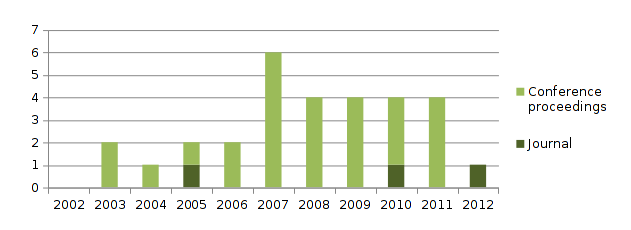
\includegraphics[width=1\textwidth]{img/Publications}
    \caption{Julkaistut tutkimukset vuosittain}
    \label{fig:publications}
  \end{center}
\end{figure}

Suurimmassa osassa julkaisuja oli ilmoitettu ajankohta, jolloin muutoksen ensi
askeleet oli otettu. Kuva~\ref{fig:start_year} esittää ilmoitetut muutosten
alkuajankohdat ryhmiteltynä vuosittain. Mediaani muutoksen aloitusajankohdasta
siitä kertoneen tutkimuksen julkaisuun oli kolme vuotta. Tämä näkyy aloitettujen
muutoshankkeiden nousussa vuonna 2004 ja julkaisujen lukumäärän nousussa vuonna
2007. Tästä voidaan päätellä, että suuren mittakaavan muutokset ketteriin
menetelmiin ovat yleistyneet viime vuosikymmenen puolesta välistä alkaen.

\begin{figure}[htb]
  \begin{center}
    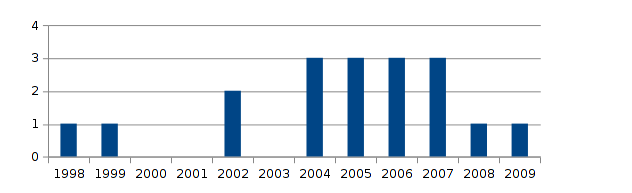
\includegraphics[width=1\textwidth]{img/Transformation_start}
    \caption{Organisaatiomuutosten aloitusajankohdat vuosittain}
    \label{fig:start_year}
  \end{center}
\end{figure}

\subsection{Käytetyt ketterät menetelmät}

Kaikkissa tapauksissa organisaatio oli raportoidun ajanjakson lopussa edelleen
jatkanut ketterien menetelien soveltamista. Muutoksen vaikutuksia oli
tyypillisesti raportoitu 1 tai 2 vuoden päähän sen aloittamisesta. Suurimmassa
osasta tapauksia muutos katsottiin edelleen jatkuvan raportin
kirjoitusajankohtana.

Suurin osa tutkimuksta erotteli käytössä olevia ketteriä menetelmiä.
Taulukko~\ref{table:practices} esittää tutkimuksissa eniten raportoidut
menetelmät. Ylivoimaisesti suosituin ketterä menetelmä oli Scrum, jota
mainittiin käytettävän miltei kahdessa kolmesta organisaatiosta. Toiseksi
suosituin menetelmä oli Extreme Programming. Osassa organisaatioista myös kevyt
kehitysmalli oli yhdistetty ketteriin menetelmiin.

Taulukosta~\ref{table:practices} ilmenee myös eri menetelmien yhdistely
huomattavana trendinä. Lähes kolmanneksessa raporteista mainittiin suoraan, että
menetelmiä oli yhdistelty. Menetelmien yhdistelemistä ja räätälöintiä oli
perusteltu pääasiallisesti kahdella tapaa. Osassa raporteista oli syyksi
mainittu se, että suuren organisaation erityispiirteet tekivät menetelmän
räätälöinnin välttämättömäksi. Toisaalta yritykset olivat halunneet panostaa
mahdollisimman hyvän menetelmän löytämiseen, jolloin useita menetelmiä oli
arvioitu ja niiden sopivimmat piirteet oli yhdistetty.

\begin{table}[h]
    \begin{tabular}{ll}
        \toprule
        Menetelmä       & N   \\ \midrule
        Scrum           & 18 \\ 
        XP              & 7 \\
        Lean            & 5 \\
        Eri menetelmien yhdistely ja räätälöinti & 9  (epäsuorasti mainittuna useampia) \\
        \bottomrule
    \end{tabular}
	\caption{Hauissa käytetyt näkökulmat ja niitä vastaavat avainsanat. Sarake N
	kuvaa kuinka monessa tutkimuksessa menetelmää mainittiin käytettävän.}
	\label{table:practices}
\end{table}

Edellä mainittujen ketterien mallien lisäksi oli yksittäisiä mainintoja
seuraavista menetelmistä: JAD (Joint Application Development),
ASSF\footnote{Qumer ja Henderson-Sellers [S9] kuvaavat ASSF-menetelmän}, Unified
Process, sekä DSDM (Dynamic Systems Development Method). Näiden menetelmien
lisäksi mainittiin erilaisia käytäntöjä, mukaan lukien ajallinen rytmittäminen,
testivetoinen kehitys, asiakkaan mukanaolo, testauksen automatisointi, sekä
jatkuva yhdentäminen.

\subsection{Perusteet organisaatiomuutoksen aloittamiselle}

\hl{--> Vaatimus parannukseen (16 kpl)}
--> Ongelmia havaittu nykyisessä mallissa (12 kpl)
--> Nopeampi TTM (10 kpl)

\hl{--> Kolmanneksessa tapauksista mainittiin}, että muutokseen ryhdyttiin
erityisesti yrityksen johdon aloitteesta.

\hl{--> Organisaatioiden} lähtötila
--> Kolmannes tutkimuksista raportoi vesiputousmallin olevan käytössä
--> Lähes puolella tutkimuksista ilmoittivat tekevänsä pitkiä (vähimmillään
vuoden mittaisia) julkaisusyklejä.

\subsection{Organisaatiomuutosten piirteet}

Ketterien menetelmien käyttöönottoon tähdänneitä organisaatiomuutoksia
tarkastellaan viidestä eri näkökulmasta, jotka ilmenivät ensisijaisista
tutkimuksista. Ensimämiset näkökulmat ovat tapa jolla muutosta johdettiin ja
malli jolla muutosta toteutettiin. Muut keskeiset näkökulmat ovat
organisaatioiden tekemät sijoitukset organisaatiomuutokseen, miten
yhteisönrakentamisella pyrittiin ankkuroimaan muutosta sekä pilotoinnin käyttö.

\subsubsection{Muutoksen johtaminen}

Organisaation johdolla on keskeinen rooli muutoksissa, mikä näkyy siinä, että
suuressa osassa ensisijaisia tutkimuksia kerrotaan, että johto oli ensimmäisenä
käynnistänyt organisaatiomuutoksen. Useassa tapauksessa johto oli myös
vetovastuussa muutoksen läpiviemisestä. Esimerkiksi Goos ja Melisse [S4]
kertovat että johdon vahva osallistuminen oli tärkeää muutoksen juurruttamiseksi
ja oikean suunnan säilyttämiseksi, vaikka toimeenpaneva vastuu uusien
käytäntöjen luomisesta oli toteuttavalla portaalla. Myös Maples [S11] kuvaa,
miten tuotekehitys oli ottanut käyttöön ketteriä malleja tiimikohtaisesti, mutta
uusien käytäntöjen yhteensovittaminen ja koordinointi koko organisaation
laajuudessa vaati aloitetta johdon tasolla.

Organisaatiomuutos vaatii tahon jolla on vahvaa halua muutokseen, johtamiskykyä
ja vaikutusvaltaa. Useassa tapauksessa muutoksessa oli yksi keskeinen henkilö,
joka toimi muutoksen mestarina (engl. champion). Muun muassa O'Connor [S6]
esittää kuinka muutos aloitettiin uuden teknologiajohtajan toimesta, jolla oli
kokemusta aikaisemmista organisaatiomuutoksista. Myös Atlas [S1] raportoi
muutosta, jossa muutosta veti yksi asialle omistautunut henkilö. Kyseisessä
tapauksesa muutoksen mestari onnistui juurruttamaan muutoksen siten, että hän
pystyi lopuksi luovuttamaan muutoksen vetovastuun organisaatioon muodostuneelle
ketteriä menetelmiä edistävälle yhteisölle [S1]. Kahdessa tapauksessa
organisaatio palkkasi ulkopuolisen konsultin vetämään muutosta [S5, S30].

Joissakin tapauksissa organisaatiomuutosta ohjasi työryhmä johon oli koottu
useita eri näkökulmia edustavia jäseniä. Bang [S17] kertoo miten muutoksen
koordinointia varten perustettiin projektiryhmä, johon kuului jäseniä muun
muassa ylemmästä johdosta, myynnistä, projektijohdosta, ohjelmistokehityksestä
ja graafisesta suunnittelusta. Poikkiorganisatoorillisen työryhmän tärkeäksi
ominaisuudeksi raportoitiin se, että kaikkien osapuolten näkemyksiä kuullaan ja
vastakkainasetteluita sillataan [S15, S19].

\subsubsection{Muutoksen malli}

Yleisin malli josta ensisijaisissa tutkimukseissa raportoitiin oli ketterien
menetelmien askeleittainen käyttöönotto. Esimerkiksi Pertersen ja Wohlin [S27]
kertovat miten askeleittainen käyttöönotto toteutettiin ottamalla ensiksi
käyttöön pienet tiimit ja tuotteen kehitysjono (engl. product backlog), ja vasta
näiden ollessa toiminnassa siirryttiin soveltamaan muita käytäntöjä kuten
jatkuvaa prosessinparannusta ja päiväpalavereita (engl. stand-up meetings).
Wilby [21] kertoo että ketterä kehityks otettiin ensin käyttöön tiimitasolla,
jonka jälkeen todettiin että pitkän tähtäimen suunnittelu pitää myös muuttaa
ketteräksi. Myös Moore ja Spens [S23] esittävät miten suunnittelu muutettiin
joustavaksi ensin yksittäisten tiimien tasolla, mikä synnytti tarpeen kehittää
tehokkaampia tapoja hallita riippuvuuksiin vaikuttavaia muutoksia ja tiimien
tuotosten yhdentämistä. Pilottiprojektit olivat myös suosittu tapa hallita
askeleittaista käyttöönottoa (katso kohta \ref{subsec:pilotointi}).

Vastakohtana askeleittaiselle käyttöönotolle eräässä organisaatiossa päädyttiin
muuttamaan kaikki kehitystiimit yhdellä kertaa käyttämään ketterää mallia.
Perusteluna yhdellä kertaa toteutetulle käyttöönotolle oli johdon pyrkimys
esittää vahvaa määrätietoisuutta muutoksessa, sekä toimintatapojen pitäminen
yhdenmukaisina. Kerralla toteutettun muutoksen raportoitiin onnistuneen. [S19]

Osassa organisaatioita muutoksen myötä päädyttiin malliin jossa yhdistettiin
aikaisempia toimintatapoja ja ketteryyttä. Esimerkiksi Karlström ja Runeson [S8]
kertovat miten ketterät menetelmät yhdistettiin Stage-Gate malliin, joka
helpotti tiimien välistä koordinointia sekä kommunikaatiota markkinoinnin ja
ylemmän johdon kanssa. Wilbyn [S21] kuvaamassa organisaatiossa alkuperäinen
vuosittainen roadmapping-käytöntö sovitettiin ketteräksi lyhentämällä
suunnitteluväliä neljännesvuoteen, ja ottamalla suunnitteluun mukaan edustajia
kaililta organisaation osa-alueilta.

\hl{--> Oleellinen muutoksen vaikuttava} tekijä oli organisaation muut toiminnot
joiden kanssa ketterät ohjelmistokehitystiimit joutuvat kommunikoimaan.
--> (13 viitettä ja esimerkkiä)

\subsubsection{Konsultointi, koulutus ja muut muutokseen liittyvät sijoitukset}

Ulkopuolisten konsulttien käyttö oli hyvin tyypillistä, ja siitä oli raportoitu
yli puolessa kaikista ensisijaisista tutkimuksista. Konsultteja käytettiin
erityisesti muutosprosessin suunnittelussa ja ketterän kehitysmallin
sovittamisessa organisaation tarpeisiin [S5, S10, S21, S23, S26, S29]. Konsultit
seurasivat usein organisaatiota läpi muutoksen ja toimivat tiimien valmentajina
(engl. coach) ketterää kehitystä varten [S4, S6, S19, S23, S30]. Konsultteja
käytettiin myös kouluttamaan organisaation sisäisiä ketterän kehityksen
valmentajia [S4, S28].

Koulutus oli keskeisessä osassa muutosta, ja suuri osa ensisijaisista
tutkimuksista raportoi siitä [S1, S5, S10, S16, S19, S22, S26, S30]. Jotkut
organisaatiot räätälöivät oman opetussuunnitelman ketterien menetelmien
kouluttamiseen. Abernathy [S16] kertoo räätälöidyn opetussuunnitelman tuottaneen
niin hyviä tuloksia, että organisaatio päätti alkaa antaa koulutusta myös
ulkopuolisille tahoille. Koulutusta vahvistettiin useassa tapauksessa
erilaisilla työpajoilla, epävirallisilla tapaamisilla ja seminaareilla.
Esimerkiksi McDowell ja Dourambeis [S7] kuvaavat miten organisaatiossa
toteutettiin useita noin sadan osallistujan päivän mittaisia tapahtumia, jossa
harjoiteltiin ketterien menetelmien käyttöä. Seffernick [S10] kertoo
työpajoista, joilla vahvistettiin projektinjohdon ja tuoteomistajien ymmärrystä
ja innokkuutta ketterän mallin käyttöön.

Muutos ketterään malliin merkitsi toimintatapojen muuttamisen lisäksi myös
fyysisten tilojen uudelleenjärjestämistä. Seffernick [S10] raportoi että
työpisteet uudelleenjärjestettiin muodostamaan tiimihuoneita, ja lisäksi
rakennettiin pelihuone ja kahvila yleisiin tiloihin. Heidenberg et al. [S26]
kertoo työtilan järjestelyn tiimihuoneiksi vieneen enemmän tilaa henkilöä kohden
kuin tavanomaisessa toimistotilassa, mikä vaati lisäresursointia.

Ketterä kehitys vaati myös panostusta uusiin työkaluihin. Esimerkiksi Fry ja
Greene [S19] sekä Ryan ja Scudiere [S29] raportoivat wiki-järjestelmän
käyttöönotosta tiedonjakamisen helpottamiseksi. Ensisijaisissa tutkimuksissa
kerrottiin myös panostuksista laadunvarmistusksen työkaluihin. Esimerkiksi Fry
ja Greene [S19] kertovat miten testausautomaation rakentaminen oli keskeisenä
tekijänä ketterien menetelmien soveltamisessa. Myös Moore ja Spens [S23]
raportoivat merkittävästä panostuksesta testaukseen sekä jatkyvan yhdentämisen
työkaluihin.

\subsubsection{Yhteisöllisyyden rakentaminen}

Yhteisöllisyyden rakentamista käsiteltiin tärkeänä asiana suuressa osassa
ensisijaisia tutkimuksia. Yhteisöllisyyden luominen uusien työtapojen ympärille
on keskeistä muutoksen juurruttamisen kannalta. Esimerkiksi Abernathy [S16]
kuvaa miten organisaatiossa pyrittiin luomaan yhteisöjä eri osaamisen, muun
muassa testauksen, arkkitehtuurin ja järjestelmäanalyysin, alueilla.
Näiden yhteisöjen tarkoitus oli levittää tietoa, osaamista ja uusia työtapoja
yli organisaation sisäisten rajojen [S16]. Atlas [S1] kertoo miten muutoksen
mestari onnistui muodostamaan yhteisön uuden toimintamallin ympärille siten,
että hän itse pystyi väistymään johtavasta roolista ketterien menetelmien
edistämisessä.

Valmentamista voidaan pitää eräänä yhteisöllisyyden muotona. Valmentaja toimii
uuden menetelmän puolestapuhujana, ja avustaa tiimejä menetelmän käytännön
soveltamisessa. Muun muassa Silva ja Doss [S28] kuvaavat miten valmentaminen oli
tärkeä toiminto ketterien menetelmien käyttöönotossa, ja miten myös valmentajat
muodostivat oman yhteisönsä. Myös Benefield [S22] mainitsee valmennuksen
tärkeyden.

\subsubsection{Pilottihankkeiden soveltaminen}
\label{subsec:pilotointi}

Pilotoinnin soveltaminen oli tyypillistä muutoksen alussa. Pilottiprojektien
keskeinen vaikutus oli myönteisen asenteen muodostuminen ketterää kehitystä
kohtaan [S4, S6, S8, S10, S24, S26, S28]. Toinen pilottiprojektien tavoite oli
uuden prosessin ja työkalujen räätälöinti ja arviointi [S4, S14, S26].
Useassa organisaatioissa suoritettiin monta pilottiprojektia [S4, S22, S24,
S28]. Syynä oli muun muassa se, että projektejen katsottiin eroavan toisistaan,
ja tarvittiin todisteita ketterien menetelmien laaja-alaisesta
sovellettavuudesta [S26]. Eräässä organisaatiossa päädyttiin suorittamaan
pilottiprojektit liiketoiminnan kannalta kriittisissä projekteissa, joihin ei
saanut aiheutua keskeytyksiä [S4].

Pilotoinnin suunnitteluun liittyi myös haasteita. O'Connor [S6] kertoo miten
erittäin suotuisan ympäristön luominen pilottiprojektille ja erinomaiset
lopputulokset loivat epärealistisia odotuksia. Tämä johti käyttöönoton
laajentuessa turhautumiseen, kun samoja tuloksia ei enää kyetty saavuttamaan.

\subsubsection{??? Muuta ???}

\hl{--> Lopputuloksena oli ketterien menetelmien} pysyvä käyttöönotto, paitsi [S5]
jossa organisaatio alkoi palata käyttämään vanhaa menetelmää. Yhdessä
tapauksessa ketterien menetelmien pilottiprojekti keskeytettiin
organisaation yleisen taloustilanteen takia [S26].

\subsection{Ongelmia ketterän kehityksen käyttöönotossa}

Onnistuneen ketterien käyttöönotossa esiintyneitä haasteita listataan neljässä
eri kategoriassa. Ensimmäiseksi käsitellään ongelmia saavuttaa hyväksyntä ja
yhtenäinen suunta muutokselle. Toisena kategoriana esitellään ketterien
menetelmien väärinymmärryksestä johtuneita ongelmia. Kolmas kategoria on
ketterän mallin soveltumattomuus ja ristiriidat organisaation eri ryhmien
välillä. Neljänneksi käsitellään haasteita jotka ovat aiheutuneet
puutteellisesta resursoinnista ja varautumisesta muutokseen.

\subsubsection{Organisaation yhtenäinen suuntaaminen muutoksessa}

Muutoksen johtamisen kannalta haasteeksi nousi usein yhtenäisen suunnan
saavuttaminen muutoksessa. Yhtenäisyyden puutteen oireiksi voidaan tulkita
johdon tuen puuttuminen, muutosvastarinta ja liika innokkuus. Hajjdiab et al.
[S5] kertovat miten johdon tuen puuttuminen vähensi henkilöstön motivaatiota
panostaa muutokseen ja hankaloitti muutokseen vaatimaa resursointia. Spayd [S13]
kuvaa, että vaikka kehittäjille oli järjestetty koulutusta, keskijohdolle ei
ollut suunniteltu sopivaa koulutusohjelmaa, jonka seurauksena ymmärryksen
puute muodostui suurimmaksi muutosta haittaavaksi tekijäksi.

Muutosvastarintaa syntyi muun muassa tiimitilojen uudelleenjärjestelystä [S14].
Hallikainen [S14] kertoo että muutosvastarintaa poistettiin suurella
panostuksella henkilökohtaisiin keskusteluihin johtajien ja henkilöstön välillä.
Heidenberg et al. [S26] kertoo että muutosvastarintaa pyrittiin lieventämään
pilotoinnilla. Benefield [S22] esittää että tilanteesta riippumatta on
hyväksyttävä ja varauduttava siihen, että 10-15 \% henkilöstöstä ei ole
tyytyväisiä käytössä oleviin toimintatapoihin.

Muutosvastarinnan vastakohtana yli-innokkuus aiheutti myös ongelmia. Muun muassa
Hajjdiab et al. [S5] sekä O'Connor [S6] kuvaa miten yli-innokkuus johti 
kiinnostuksen menettämiseen ja turhautumiseen. Benefield [S22] kuvaa miten
ketterien menetelmien valmentajia piti ohjata välttämään menetelmien
määräämistä, ja sen sijaan antamaan suosituksia, jotta heitä ei tulkittaisi
yli-innokkaiksi ja epäuskottaviksi.

Useassa tapauksessa ketterää muutosta uhkasi vanhan toimintamallin palaaminen.
Muun muassa Goos ja Melisse [S4] kertoivat kehittäjien palaavan
aikatalulupaineen alla käyttämään vanhasta mallista tuttuja käytäntöjä. Myös
arkkitehtuurilliset yhdentämisvaikeudet eri osastojen välillä johtivat
sopimuspohjaisen menettelyn paluuseen [S23]. Maples [S11] kuvasi että tuotteen
julkaisuprosessia ei oltu muutettu ketteräksi, ja se vaati julkaistavien
ominaisuuksien lukitsemisen 90 päivää etukäteen. Ominaisuuksien lukitseminen
aiheutti määräilevän johtamistyylin paluuta, mikä soti ketteriä periaatteita
vastaan [S11].

\subsubsection{Uuden mallin väärinymmärtäminen}

Ketterien menetelmien soveltaminen väärin oli yleinen ongelma. Esimerkiksi
Benefield [S22] kuvaa miten koulutuksen resurssipulan takia jotkut tiimit
väittivät käyttävänsä ketteriä menetelmiä, mutta tekivät todellisuudessa
pienoiskokoista vesiputouskehitystä. Projektipäälliköt käyttivät myös
Scrum-termistöä, mutta todellisuudessa jakoivat työtehtäviä määräilevästi, ja
tekivät sitoumuksia kuulematta tiimiä [S22]. Myös Seffernick [S10] kuvaa miten
vanhan mallin rooleja sovitettiin Scrum-malliin muuttamatta toimintatapoja, mikä
ei edistänyt toimintamallin muutosta. Maples [S11] kertoo miten kaikkien
osapuolten kuuleminen ymmärrettiin väärin siten, että tuotteen kehitysjonoon
tulvi liikaa vaatimuksia, mikä johti vaatimusten kauppaamiseen ja
epätehokkaaseen priorisointiin. Abernathy [S16] kuvaa miten linjajohtajat
puuttuivat tiimien sisäisiin asioihin, mikä johti luottamuspulaan ja haittasi
ketterän mallin toteuttamista.

\subsubsection{Soveltuvuus ja ristiriidat organisaation muiden ryhmien kanssa}

Monessa tapauksessa ketterä kehitys saatiin toimimaan yksittäisten tiimien
tasolla, mutta ongelmia alkoi esiintyä kun ketterää mallia alettiin soveltaa
laajemmin. Maples [S11] kertoo, että markkinointiosasto joutui törmäyskurssille
tuotekehityksen kanssa kun ketterien menetelmien käyttöä laajennettiin, sillä
vanhassa kehitysmallissa markkinointi vaati suunnitelmien lukkoonlyömistä
pitkällä tähtäimellä. Myös vientilupien ja kolmannen osapuolen lisenssien
hankkiminen vaati suunnittelua pidemmällä aikavälillä. Lopputuloksena
muodostettiin malli jossa markkinoinnin sallitaan määrittää julkaisupäivä tietty
aika etukäteen, ja tuotekehitys sitoutuu toimittamaan tietyt toiminnallisuudet
siihen mennessä [S11]. Myös O'Connor [S6] kertoo kuinka organisaation johto
vaati pidemmän tähtäimen suunnitelmia, joita oli ongelmallisia toimittaa
ketterän kehityksen puitteissa. Eräässä tapauksessa johto ja myyntiosasto
tukivat ketterää kehitystä pyrkimällä päivittämällä sopimuskäytäntöjä sallimaan
ketteryyttä paremmin [S17]. Moore ja Spens [S23] kertovat kuinka ketterässä
kehityksessä käytetty joustavampi suunnittelu toi muutoksia, jotka aiheuttivat
laatuongelmia kun projektien tuotoksia yhdennettiin.

Joissakin organisaatioissa havaittiin, että ketterä kehitys ei sovellu
laajennettavaksi kaikkiin toimintoihin. Muun muassa Korhonen [S2] kertoo että
Scrum-käytännöt eivät soveltuneet testaukseen ja tukitoimintoihin. Tukitiimin
toimintatapa vaati välitöntä vastaamista ongelmiin, eikä ajallisen rytmittämisen
periaatteita voitu soveltaa [S2]. Myös Spayd [S13] esitti ketterien mallien
havaittiin soveltuvan huonosti ylläpitokehitykseen. Ylläpitotiimit samaistuivat
kuitenkin käynnissä olevaan muutokseen, ja menetelmien tarkempi räätälöinti
jätettiin tulevaisuuteen [S13]. Goos ja Melisse [S4] havaitsivat että ketterät
menetelmät soveltuivat organisaation toimintoihin sitä huonommin mitä kauempana
tuotekehityksestä ne oli.

Benefield [S22] raportoi että organisaation hallinto-osastot kuten
henkilöstöhallinto ja matriisiorganisaation johto asettivat toimintatavoillaan
haasteita ketterälle kehitykselle. Edellä mainitut osastot pyrkivät
hallinnoimaan työntekijöitä yksilötasolla, mikä haittasi ketterien menetelmien
tiimikeskeistä toimintatapaa [S22]. Spayd [S13] kertoo kuinka henkilöstöhallinto
esti tiimikohtaisen palkitsemisen, sekä tilahallinto esti tiimejä muodostamasta
yhteisiä tiloja.

\subsubsection{Puutteellinen varautuminen muutokseen}

Suurimmaksi resursointiongelmaksi muodostui valmennuksen ja koulutuksen puute.
Esimerkiksi Benefield [S22] raportoi että osaavien valmentajien puute hidasti
ketterien menetelmien käyttöönoton laajentamista. Silva ja Doss [S28]
käsittelevät haasteita uusien valmentajien koulutuksessa, kun valmennuksen tarve
kasvoi voimakkaasti uuden kehitysmallin yleistyessä. Valmentajakoulutukseen
hakeutuneet henkilöt olivat usein tottuneita perinteiseen ohjelmistokehityksen
malliin, mikä aiheutti riskin, että uudet valmentajat olisivat levittäneet
väärin käsitettyä ketterän kehityksen mallia [S28]. Myös Spayd [S13] raportoi
puutteellisesta koulutuksesta, jonka takia ketteriä periaatteita ei ymmärretty
ja sovellettiin epätehokkaasti.

\subsection{Muutosprosessin menestyksen tekijät}

Ensisijaisista tutkimuksista tunnistettiin neljä tekijää jotka edesauttoivat
muutosprosessin menestystä. Ensimmäinen tekijä on organisaation yhdenmukainen
suuntaaminen ja muutoksen johtaminen. Muutoksen suunnitteleminen on toinen
tekijä joka esitellään. Kolmanneksi esitellään hyviä käytäntöjä uuden
toimintatavan soveltamisessa. Neljäntenä tekijänä on riittävä resursointi
muutoksen läpiviemiseen.

\subsubsection{Organisaation yhdensuuntaistaminen ja muutoksen johtaminen}

--> Johdon tuki (5 viitettä)
--> Johdon tulee välttää muutokseen pakottamista (4 viitettä)

--> Muutosta johtavan tahon tulee toiminnallaan lisätä ketterien menetelmien
kannatusta (5 viitettä)

--> Muutosprosessiin on hyvä ottaa mukaan kaikki asianomaiset tahot (7 viitettä)

--> Organisaatiossa suunnan ja tavoitteiden tehokas kommunikointi on keskeinen
menestyksen tekijä. (3 viitettä)

\subsubsection{Muutoksen suunnittelminen ja seuraaminen}

Muutoksessa on oleellista tunnistaa muutoksen tärkeimmät osa-alueet ja keskittyä
niihin ensin. (3 viitettä)

--> Muutoksesta voi tehdä suunnitelman (mikä on hyvä suunnitelma?) (3 viitettä)

--> Muutosta kannattaa tarkkailla, ja toiminnan tehokkuutta mitata (4 viitettä)

\subsubsection{Ketterän menetelmän onnistunut soveltaminen}

--> Suunnittele johdon ja esimiesasemissa olevien henkilöiden tehtävät
(3 viitettä)

--> Toteuttavast portaasta lähtevä menetelmien soveltaminen (4 viitettä).

--> Menetelmien soveltaminen (5 viitettä).

Useassa tapauksesa raportoitiin yhdenmukaisten toimintatapojen eduista.
(8 viitettä)
--> Yhdenmukaisuuden katsottiin oleelliseksi tekijäksi useassa organisaatiossa.
Yhdenmukaisuudella pyrittiin muun muassa vertailukelpoisuuteen eri projektien
välillä [???]. Suuressa organisaatiossa on eri toimintojen välisessä
kommunikaatiossa hyötyä yhteisestä sanastosta [???].

\subsubsection{Muutokseen sijottaminen}

--> Ulkopuolisten resurssien hyödyntäminen. (2 viitettä)

--> Koulutus (6 viitettä)

--> Työkaluihin ja ympäristöön sijoittaminen (2 viitettä)
--> CI ja automaatio (1 viite)

% --------------------------------------------------------------------
\clearpage
\section{Johtopäätökset ja yhteenveto}
\label{sec:johtopaatokset}

--> Muistutus työon tavoitteista (sidoksisuus johdantoon)

--> Yhteenveto tuloksista, ja tulosten merkitys
--> Suositus toimnepiteisiin??

--> Ei vertailtu pienten organisaatioiden ketterään käyttöönottoon.
--> Mitkä olivat erityiset tekijät jotka erosivat
--> Spekulatiivinen vastaus

--> Tulosten soveltuvuus
--> Tutkimuksen arviointi

--> Lisätutkimuskysymyksiä jatkoa varten: käyttöönoton laajuus /
oerganisaatiotyypit / mitkä menetelmät / enemmän perusteita miksi ?? 

--> Jatkotutkimukset
--> Pitää tehdä kirjallisuustutkimus seuraten huolellisesti jotakin
kijallisuustutkimuksen menetelmää. Jotta sain järjestelmällisen
kirjallisuustutkimuksen sovitettua kandidaatintyön laajuuteen jouduin
karsimaan useita oleellisia menetelmään kuuluvia muodollisuuksia.



\label{pages:text}
\clearpage


% -------------- Lähdeluettelo / reference list ----------------------

% Viitetyylitiedosto aaltosci_t.bst; muokattu HY:n tktl-tyylistä.
\bibliographystyle{aaltosci_t}
\bibliographystylepri{aaltosci_t}

% Muutetaan otsikko "Kirjallisuutta" -> "Lähteet"
\renewcommand{\refname}{Lähteet}  % article-tyyppisen
%\renewcommand{\bibname}{Lähteet}  % jos olisi book, report-tyyppinen

\addcontentsline{toc}{section}{\refname}  % article
%\addcontentsline{toc}{chapter}{\bibname}  % book, report

\bibliographypri{lahteet}

\nobibliography{lahteet_s}

\clearpage

\section*{Ensisijaiset tutkimukset}
\addcontentsline{toc}{section}{Ensisijaiset tutkimukset}  


\begin{supertabular}{ l p{14.2cm} }
    {[S1]} & \bibentry{S1} \\ 
    {[S2]} & \bibentry{S2} \\ 
    {[S3]} & \bibentry{S3} \\ 
    {[S4]} & \bibentry{S4} \\ 
    {[S5]} & \bibentry{S5} \\ 
    {[S6]} & \bibentry{S6} \\ 
    {[S7]} & \bibentry{S7} \\ 
    {[S8]} & \bibentry{S8} \\ 
    {[S9]} & \bibentry{S9} \\ 
    {[S10]} & \bibentry{S10} \\ 
    {[S11]} & \bibentry{S11} \\ 
    {[S12]} & \bibentry{S12} \\ 
    {[S13]} & \bibentry{S13} \\ 
    {[S14]} & \bibentry{S14} \\ 
    {[S15]} & \bibentry{S15} \\ 
    {[S16]} & \bibentry{S16} \\ 
    {[S17]} & \bibentry{S17} \\ 
    {[S18]} & \bibentry{S18} \\ 
    {[S19]} & \bibentry{S19} \\ 
    {[S20]} & \bibentry{S20} \\ 
    {[S21]} & \bibentry{S21} \\ 
    {[S22]} & \bibentry{S22} \\ 
    {[S23]} & \bibentry{S23} \\ 
    {[S24]} & \bibentry{S24} \\ 
    {[S25]} & \bibentry{S25} \\ 
    {[S26]} & \bibentry{S26} \\ 
    {[S27]} & \bibentry{S27} \\ 
    {[S28]} & \bibentry{S28} \\ 
    {[S29]} & \bibentry{S29} \\ 
    {[S30]} & \bibentry{S30} \\ 
\end{supertabular}

%\bibliographysec{lahteet_s}


\label{pages:refs}
\clearpage         % erotetaan mahd. liitteet alkamaan uudelta sivulta


% -------------- Liitteet / Appendices --------------------------------
%
%\appendix
%\input{luku_liitteet}
%\label{pages:appendices}


% ---------------------------------------------------------------------

\end{document}
